%\setcounter{chapter}{1}
\chapter{Luyện tập: Công và Công suất}
\begin{enumerate}
	\item %câu 1
	Công là đại lượng
	\begin{mcq}(1)
		\item vô hướng có thể âm, dương hoặc bằng không.
		\item vô hướng có thể âm hoặc dương.
		\item vectơ có thể âm, dương hoặc bằng không.
		\item vectơ có thể âm hoặc dương.
	\end{mcq}
	\item %câu 2
	Vật nào sau đây không có khả năng sinh công?
	\begin{mcq}(1)
		\item Dòng nước lũ đang chảy mạnh.
		\item Viên đạn đang bay.
		\item Búa máy đang rơi xuống.
		\item Hòn đá đang nằm trên mặt đất.
	\end{mcq}
	\item %câu 3
	Một vật chịu tác dụng của một lực $F$ không đổi có độ lớn $\SI{5}{\newton}$, phương của lực hợp với phương chuyển động một góc $60^\circ$. Biết rằng quãng đường đi được là $\SI{6}{\meter}$. Công của lực $F$ là
	\begin{mcq}(4)
		\item $\SI{11}{\joule}$.
		\item $\SI{50}{\joule}$.
		\item $\SI{30}{\joule}$.
		\item $\SI{15}{\joule}$.
	\end{mcq}
	\item %câu 4
	Một vật khối lượng $m=\SI{10}{\kilogram}$ được kéo chuyển động thẳng nhanh dần dều trên sàn nhẵn không ma sát bằng một lực $F=\SI{5}{\newton}$ theo phương ngang từ trạng thái nghỉ. Trong thời gian 4 giây tính từ lúc bắt đầu chuyển động công suất trung bình của lực $F$ bằng
	\begin{mcq}(4)
		\item $\SI{10}{\watt}$.
		\item $\SI{8}{\watt}$.
		\item $\SI{5}{\watt}$.
		\item $\SI{4}{\watt}$.
	\end{mcq}
	\item %câu 5
	Một người kéo một vật có $m=\SI{8}{\kilogram}$ trượt trên mặt phẳng ngang có hệ số ma sát $\mu=0,2$ bằng một sợi dây có phương hợp một góc $60^\circ$ so với phương nằm ngang. Lực tác dụng lên dây bằng $\vec{F}_\text{k}$ vật trượt không vận tốc đầu với $a=\SI{1}{\meter/\second^2}$. Công của lực kéo trong thời gian 4 giây kể từ khi bắt đầu chuyển động là
	\begin{mcq}(4)
		\item $\SI{162,5}{\joule}$.
		\item $\SI{140,7}{\joule}$.
		\item $\SI{147,5}{\joule}$.
		\item $\SI{126,7}{\joule}$.
	\end{mcq}
	\item %câu 6
	Một vật có khối lượng $m=\SI{3}{\kilogram}$ được kéo lên trên mặt phẳng nghiêng một góc $30^\circ$ so với phương ngang bởi một lực không đổi $F=\SI{70}{\newton}$ dọc theo mặt phẳng nghiêng. Biết hệ số ma sát là 0,05, lấy $g=\SI{10}{\meter/\second^2}$. Tổng công của tất cả các lực tác dụng lên vật là $\SI{215}{\joule}$.
	\begin{center}
		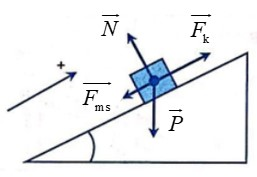
\includegraphics[scale=0.8]{../figs/VN10-PH-30-P-022-1-H2.jpg}
	\end{center}
	Quãng đường tương ứng vật đã di chuyển bằng
	\begin{mcq}(4)
		\item $\SI{1}{\meter}$.
		\item $\SI{2}{\meter}$.
		\item $\SI{4}{\meter}$.
		\item $\SI{6}{\meter}$.
	\end{mcq}
	\item %câu 7
	Một vật có khối lượng $m=\SI{500}{\gram}$ trượt từ đỉnh B đến chân C của một mặt phẳng nghiêng có chiều dài $l=\text{BC}=\SI{2}{\meter}$, góc nghiêng $\beta$; $g=\SI{10}{\meter/\second^2}$. Công của trọng lực thực hiện khi vật di chuyển từ B đến C bằng $\SI{4}{\joule}$.
	\begin{center}
		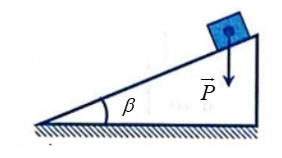
\includegraphics[scale=0.8]{../figs/VN10-PH-30-P-022-1-H1.jpg}
	\end{center}
	Giá trị của $\beta$ bằng
	\begin{mcq}(4)
		\item $30^\circ$.
		\item $31^\circ$.
		\item $51^\circ$.
		\item $24^\circ$.
	\end{mcq}
	\item %câu 8
	Một ô tô có khối lượng 1,2 tấn chuyển động đều trên mặt đường nằm ngang với vận tốc $v=\SI{36}{\kilo\meter/\hour}$. Hỏi phải thực hiện một công là bao nhiêu để hãm xe dừng lại.
	\item %câu 9
	\begin{enumerate}[label=\alph*)]
		\item Tính công và công suất của một người kéo một thùng nước có khối lượng $\SI{12}{\kilogram}$ từ giếng sâu $\SI{8}{\meter}$ lên trong 16 giây? Xem như thùng nước chuyển động đều.
		\item Nếu dùng máy kéo thùng nước nói trên đi lên nhanh dần đều và sau $\SI{2}{\second}$ đã kéo lên thì công và công suất của máy bằng bao nhiêu? Tính công suất của máy khi đó.
	\end{enumerate}
	\item %câu 10
	Một xe tải có khối lượng 2,5 tấn bắt đầu chuyển động thẳng nhanh dần đều. sau khi đi được quãng đường $\SI{144}{\meter}$ thì xe đạt vận tốc $\SI{12}{\meter/\second}$. Biết hệ số ma sát giữa xe và mặt đường là $\mu=0,04$. Lấy $g= \SI{10}{\meter/\second^2}$.
	\begin{enumerate}[label=\alph*)]
		\item Tính công của các lực tác dụng lên xe trên quãng đường $\SI{144}{\meter}$ đầu tiên.
		\item Tính công suất của lực do động cơ xe hoạt động ở quãng đường nói trên.
		\item Hiệu suất hoạt động của động cơ xe tải.
	\end{enumerate}
\end{enumerate}

\textbf{ĐÁP ÁN:}
\begin{longtable}[\textwidth]{|m{0.1\textwidth}|m{0.1\textwidth}|m{0.12\textwidth}|m{0.2\textwidth}|m{0.2\textwidth}|}
	% --- first head
	\hline%\hspace{2 pt}
	\multicolumn{1}{|c}{\textbf{Câu 1}} &
	\multicolumn{1}{|c|}{\textbf{Câu 2}}& 
	\multicolumn{1}{c|}{\textbf{Câu 3}} &
	\multicolumn{1}{c|}{\textbf{Câu 4}} &
	\multicolumn{1}{c|}{\textbf{Câu 5}}  \\
	\hline
	A. &
	A. &
	D. &
	C. &
	B.\\
	\hline
	\multicolumn{1}{|c}{\textbf{Câu 6}} &
	\multicolumn{1}{|c|}{\textbf{Câu 7}}&  
	\multicolumn{1}{c|}{\textbf{Câu 8}} &
	\multicolumn{1}{c|}{\textbf{Câu 9}} &
	\multicolumn{1}{c|}{\textbf{Câu 10}} \\
	\hline
	C. &
	D. &
	$\SI{120000}{\joule}$. &
	\begin{enumerate}[label=\alph*)]
		\item $\SI{96}{\joule}$, $\SI{6}{\watt}$.
		\item $\SI{672}{\watt}$.
	\end{enumerate} &
	\begin{enumerate}[label=\alph*)]
		\item $\SI{3,24e5}{\joule}$.
		\item $\SI{13500}{\joule}$.
	\end{enumerate}\\
	\hline
\end{longtable}